\chapter{Causes of variability in estimates of mutational variance from mutation accumulation experiments} 
 \vspace{2cm}
\section{Abstract} 
Characteristics of the new phenotypic variation introduced via mutation have broad implications in evolutionary and medical genetics. Standardised estimates of this mutational variance, $V_M$, span two orders of magnitude, but the causes of this remain poorly resolved. We investigated estimate heterogeneity using two approaches. First, meta-analyses of $\sim150$ estimates from 37 mutation accumulation (MA) studies did not support a difference among taxa (which differ in mutation rate) in standardised $V_M$, but provided equivocal support for standardised $V_M$ to vary with trait type (life history versus morphology, predicted to differ in mutation rate). Notably, several experimental factors were confounded with taxon and trait, and further empirical data are required to resolve their influences. Second, we analysed morphological data from an experiment in \textit{Drosophila serrata} to determine the potential for unintentional heterogeneity among environments in which phenotypes were measured (i.e., among laboratories or time points) or transient segregation of mutations within MA lines to affect standardised $V_M$. Approximating the size of an average MA experiment, variability among repeated estimates of (accumulated) mutational variance was comparable to variation among published estimates of standardised $V_M$ for morphological traits. This heterogeneity was (partially) attributable to unintended environmental variation or within line segregation of mutations only for wing size, not wing shape traits. We conclude that sampling error contributed substantial variation within this experiment, and infer that it will also contribute substantially to differences among published estimates. We suggest a logistically permissive approach to improve the precision of estimates, and consequently our understanding of the dynamics of mutational variance of quantitative traits. \par 

\newpage
 	 
\section{Introduction}
The magnitude of per-generational increase in genetic variance due to spontaneous mutations ($V_M$) is important for a wide range of genetic and evolutionary phenomena, including the maintenance of quantitative genetic variance \citep{Lync88b, Bart89, John05}. Much of our understanding of $V_M$ comes from mutation accumulation (MA) experiments, where populations diverge phenotypically due solely to the neutral fixation of new mutations \citep{Muka64,Hall09}. Reviews of MA experiments in a range of traits and taxa have reported that mutation increases phenotypic variance in quantitative traits by $10^{-4}$ to $10^{-2}$ times the environmental variance of the trait, or 0.02 to 5.1 percent of the trait mean per generation \citep{Houl96, Lync99, Hall09}. Differences in $V_M$ may cause differences in the magnitude of standing quantitative genetic variation and, ultimately, in rates of phenotypic evolution \citep{Houl98,Lync99,Houl17,Wals18c28}. However, the causes of variation among estimates of $V_M$, and thus the evolutionary interpretation of this variability, are not well resolved.\par

Mutation rate is known to vary widely among species (reviewed in \citealp{Katj19}), with further opportunity for differences in per-generation mutation number arising through differences in ploidy, genome size, and/or effective population size \citep{Lync99,Lync10,Sung12}. Marked variation in mutation rate has also been observed within species, both among replicated MA experiments (i.e., different founder genotypes: \citealp{Ness12,Sung12,Schr13, Ho20} and among lines within a single MA panel \citep{Huan16,Ho20}. Resulting differences in mutation number may explain variation in $V_M$ estimates, such as, for example, the fourfold range of $h_M^2$ of body size estimated for different MA in \textit{Caenorhabditis elegans} \citep{Azev02, Este05, Ostr07}.\par

Traits have also been hypothesised to differ in magnitude of $V_M$ due to differences in mutation rate, arising due to differences in the number of contributing loci. Specifically, life history traits are hypothesised to be affected by more loci than morphological traits \citep{Houl91,Houl92a, Houl96, Houl98, Meri99}. The magnitude of $V_M$ depends not only on the rate of mutation, but also on their effects, and the relationship between rate and effect size is not well characterised. \citet{Besn20} demonstrated that the high mutational variance (and relatively rapid evolution) of a vulval phenotype in nematodes was due to a broad mutational target size, rather than large-effect mutation. Whether trait types differ systematically in mutational target size is difficult to assess, as a full catalogue of causal loci is unknown for most quantitative traits \citep{Bart02,Mack09,Yang10, Rock12}. Indeed, emerging evidence that diverse traits, including morphology, are all highly polygenic \citep{Yang10,Boyl17} suggests that differences in the distribution of mutational effect sizes \citep{Simo18}, rather than simply in number of contributing loci, might cause heterogeneity in estimates of $V_M$ among traits.\par

Comparison among trait types is complicated by differences among them in variability and measurement scale, which may influence standardised values. Low mutational heritability ($h_M^2$ = $V_M$/ $V_E$, where $V_E$ is the environmental variance) of life history traits relative to morphological traits has been attributed to greater environmental variance (larger $V_E$) for life history traits, rather than lower $V_M$ \citep{Houl96}. Thus, comparison on the coefficient of mutational variance scale ($CV_M$; $100 \times \sqrt{V_M}/\bar{X}$, where $\bar{X}$ is the trait mean) reveals a different picture, one of greater mutational variance in life history than morphological traits, consistent with the prediction of greater mutational target size \citep{Houl96}.\par

Other contributions to variation in magnitude of $V_M$ might be revealed by consideration of the MA experimental design itself. The timeframe over which mutations accumulate might influence estimates of $V_M$. When MA lines are established from a homozygous (heterozygous) base population, estimates of $V_M$ will be downwardly (upwardly) biased before $6N_e$ generations \citep{Lync86}. However, $V_M$ is typically estimated after $> 6N_e$ generations, suggesting limited contribution of ancestral variation to variability of $V_M$. Conversely, long-running MA experiments might underestimate $V_M$ when the cumulative effect of low fitness mutation causes line extinction, or within-line selection against further accumulation \citep{Lync99,Este04,McGu13}. A decline in $V_M$ over time has been observed in some studies \citep{Mack95}, but not in others \citep{Garc00,Hall08}.\par

Stochastic sampling from the distribution of mutational effects could also introduce temporal heterogeneity among estimates of $V_M$. For example, among-line variance estimated before versus after a line(s) fixed a large effect mutation(s) could result in inference of a much larger per generation increase in variance at the second time-point relative to the first. Transient within-line segregation of mutations might generate variability in estimates, for example causing temporary inflation of within-line variance ($V_E$), impacting power to detect among-line variance, and potentially biasing estimates of $h^2_M$ (downward) and $CV_M$ (upward; see \citealp{Hoff16}). Notably, several studies in nematode have suggested that within-line variance increased over the duration of the MA experiment \citep{Baer08,Baer10a,Brae10}, which may contribute to a pattern of lower estimated $V_M$ in longer-running MA experiments. \par

Environmental context within which MA lines are assayed could also contribute to variation among $V_M$ estimates. Several studies have considered the effect of replicable, experimenter-imposed, changes in the environment, including in temperature \citep{Wayn98}, light \citep{Kava05} and density \citep{Fry96}. Although the magnitude of $V_M$ often varies under such environmental manipulations, there is only weak evidence for predicable patterns, such as novel or stressful environments increasing the magnitude of $V_M$ \citep{Kond94,Mart06}. Even in carefully controlled laboratory experiments, factors such as food quality or quantity, light, humidity and diurnal timing of collection will vary among individuals or lines within a phenotyping assay, and among assays conducted in different laboratories or at different times within the same laboratory. Such variation may impact estimates of standardized $V_M$ through inflation of within-line variance, similar to the effect of transient, within-line segregation of new mutations. Furthermore, if MA lines differ in their response to this unintended environmental heterogeneity, then genotype by environment (G$\times$E) variance could contribute variation among MA lines, and variability among estimates of $V_M$, a potential source of variation that has received little attention (but see \citealp{Garc00}).\par

Here, we combined two approaches to investigate causes of variability in estimates of mutational variance. Given that it has been over twenty years since this variability has been broadly documented and investigated \citep{Houl96, Houl98,Lync99}, we first conducted a meta-analysis to update tests of the previously implicated causal factors of taxon \citep{Lync98, Lync99, Hall09} and trait type \citep{Houl96, Houl98}. We had intended to examine how the number of generations affected $V_M$ \citep{Lync86,Mack95}, but MA duration was strongly confounded with taxon (detailed in the Results). Second, we conducted a new empirical experiment in \textit{Drosophila serrata}, in which we repeatedly estimate the among-line (mutational) variance to investigate whether unintended environmental heterogeneity, or transient within-line segregation of mutations can contribute variation among estimates. After accounting for these effects within the data, we finally quantify the magnitude of variation among estimates from a set of 10 wing shape traits to characterise the magnitude of variation among estimates within a trait category.\par

\section{Methods} 
\subsection{Meta-analysis of empirical estimates of mutational variance} 
\subsubsection{Literature search} 
We extracted all papers in seven reviews of mutational variance: \citet{Lync88b,Keig93,Houl96,Lync98c12,Lync99,Hall09, Wals18c12}. We then searched the Web of Science database on the 11/12/2019 at 4:38 PM AEST for journal article document types meeting the topic criteria of "mutation accumulation" and (varia* or "mutat* coefficient*") and published between 1998 and 2019. These years overlapped \citet{Hall09} (fitness traits only) and \citet{Wals18c12} (brief update on \citealp{Lync98c12}), allowing us to capture papers that may have been excluded from those reviews, as well as those published subsequently. \par
Further details on the papers identified and preliminary handling steps can be found in Figure~\ref{fig:PRISM}. For 473 unique papers identified, we screened titles and abstracts, then the full text, for relevance, applying four strict criteria, retaining only studies where the estimates of mutational variance were: 1) quantitative; 2) from spontaneous MA; 3) from MA environmental conditions and; 4) not rereporting of previously published estimates. We excluded six studies of transcriptomic data as the number of traits was much larger than for other trait categories.\par

\subsubsection{Meta-analysis data collection}
For each of the 65 papers retained after applying the above criteria, mutational parameter estimates were extracted (as described in Table \ref{tab:TabS1}), associated with taxon and trait identifiers, and details of the experimental design. Twenty papers not reporting error for the mutational parameters were excluded (Table \ref{tab:TabS1}.C). Following initial qualitative assessments of data, we excluded five studies (15 traits) due to low representation of taxon type (one vertebrate,\textit{Mus musculus}; one alga, \textit{Chlamydomonas reinhardtii}, and; two non-Drosophila insects: \textit{Daktulosphaira vitifoliae} and \textit{Nasonia vitripennis}), and one study due to low representation of trait type: mitotic cell division traits (Table \ref{tab:TabS1}B). \par

Where possible, we extracted (or calculated from provided information) both the coefficient of variance ($CV_M$; 100 $\times \sqrt{V_M}/ \bar{X}$, where $\bar{X}$ is the trait mean) and mutational heritability ($h_M^2$; $V_M$/$V_E$, where $V_E$ is the environmental variance) for each trait. As detailed below, estimates were weighted by the inverse of their standard error (SE) in the meta-analysis. Where these were not reported for $h_M^2$ or $CV_M$, but were for $V_M$ and $V_E$ or $\bar{X}$, we used a sampling approach to obtain estimates. We sampled from $N \sim (\hat\theta, V)$ 10,000 times, using the \textit{rnorm} function in R [v. 3.6.1], where	$\hat\theta$ and $V$ were respectively the reported parameter value and its standard error. We then calculated $CV_M$ or $h_M^2$ for each of these simulated samples, and obtained the standard error of this sample of estimates. Samples with negative values of $V_M$ are undefined for $CV_M$; to ensure unbiased estimates of the magnitude of error we calculated $CV_M$ as: $ 100 \times$ (sign of $V_M$) $\times \left|\sqrt{V_M}\right|/ \bar{X}$. This sampling approach was used to estimate the error for 28\% of the $h_M^2$ estimates and 61\% of the $CV_M$ estimates analysed (Table \ref{tab:TabS1}A). Two studies (17 estimates) were excluded due to nonsensically large standard error estimates, while a further three estimates (from three studies) were excluded due nonsensical scaled parameter estimates (detailed in Table \ref{tab:TabS1}B). Two extreme values ($> 3$ SD) of $h_M^2$ and two of $CV_M$ were excluded from the analyses (Table \ref{tab:TabS1}B). There were 11 cases with extremely small SE (> 5 IQR below the median); notably, for six of these came from studies where confidence intervals were constrained to be positive, suggesting that this boundary condition had reduced the SE estimate, inflating metaanalysis weights for traits where the mutational variance was not supported. These outliers were excluded from analyses, although results and conclusions were qualitatively consistent when they were included.\par

\subsubsection{Predictor variables for the meta-analysis}
Estimates came from 11 species, and based on the distribution of estimates, we defined five taxon categories (Figure \ref{fig:Pies}A): Daphnia (\textit{Daphnia pulex} only); Drosophila (\textit{Drosophila melanogaster} [$n = 68$] and \textit{D. serrata} [$n = 5$]); Plant (\textit{Arabidopsis thaliana} [$n = 12$], \textit{Amsinckia douglasiana} [$n = 2$] and \textit{Amsinckia gloriosa} [$n = 1$]) and; Nematode (\textit{Caenorhabditis elegans} [$n = 62$], \textit{C. brenneri} [$n = 4$], \textit{C. briggsae} [$n = 8$], \textit{C. remanei} [$n = 5$] and \textit{Oscheius myriophila} [$n = 5$]). We differ from a previous study (\citealp{Houl96};1998) in considering size of juveniles as morphological (not growth) traits. Reflecting more recent publications, we defined a physiology category (33\% of estimates; Figure \ref{fig:Pies}B), which included locomotive, enzymatic and metabolic activity traits (Table \ref{tab:TraitTypes}), which may differ from life-history or morphological traits in mutational target size or environmental sensitivity. We assigned the relatively well-represented life history traits (52\% of estimates; Figure \ref{fig:Pies}B) into more narrowly defined sub-categories: total fitness, survival, productivity, and a miscellaneous category (capturing traits such as development time, phenology, longevity and mating success, which were individually less well represented) (Figure \ref{fig:Pies}B; Table \ref{tab:TraitTypes}).\par

\subsubsection{Meta-analyses of mutational variance estimates}
We implemented a mixed model analyses via PROC MIXED in SAS v.9.4 (SAS Institute Inc., Cary, N.C.), using restricted-maximum likelihood (REML) and applying the Satterthwaite approximation to correct the denominator degrees of freedom, to fit the model: \par
\begin{equation}
\label{eqn:metaMM}
y_{ijkl}=\mu + Taxon_i + Trait_j + Study_k + \varepsilon_{ijkl}
\end{equation}
\noindent where $y$ is the vector of published estimates (either $h_M^2$ or $CV_M$), and $\mu$ was the grand mean; the categorical predictors of taxon and trait (defined above) were fit as fixed effects. Estimates were weighted by the inverse of the standard error (SE) of $h_M^2$ or $CV_M$, obtained as detailed above. Study was fit as a random effect, accounting for non-independence among estimates within a paper (1–29 estimates per study; median = 3). Studies reporting multiple estimates varied widely in whether these were estimates from different trait types, species (strains), sexes, or time points. Likely reflecting this, most variation not accounted for by the fixed effects was observed at the residual, not study, level (99\% for $h_M^2$ ; 85\% for $CV_M$). Similarly, while some studies shared the same MA lines (Table \ref{tab:MetaNonIndepend}) fitting a further random effect to account for this non-independence did not explain any variation, a likely consequence of both the unbalanced design (only some studies share lines), and the relative variation of estimates. We investigated different options for fitting heterogenous residuals (e.g., allowing separate estimation of residuals for studies grouped depending on the number of estimates reported), but interpretation of the fixed effects (taxon and trait) were consistent across all investigated models, and we report results only from model (\ref{eqn:metaMM}) above. \par

\subsection{Variation in estimates of among-line variance within the same taxon and trait type: An experiment in \textit{Drosophila serrata}} 
To what extent do differences in magnitude among estimates of $V_M$ reflect differences in mutation number and/or effect sizes (correlated with the above-investigated proxies of taxon and trait), versus factors such as mutations segregating within MA lines or environmental dependency of mutational effects? We conducted a further experiment to address this question. \textit{Drosophila serrata} is a member of the \textit{montium} species group, endemic to Australia and Papua New Guinea, which has been extensively used in quantitative genetic research, including study of mutational variance (e.g., \citealp{McGu13,Hine18, Duga21}. A panel of 200 MA lines were founded from one of the \textit{D. serrata} Reference Genome Panel (DsRGP) lines described in \citet{Redd18}. These MA lines were each maintained by brother-sister inbreeding for 20 generations, following protocols established by \citet{McGu11a} to minimise selection. Genome-wide heterozygosity was very low (0.3\%) in the DsRGP line that founded the MA lines, and among-line variance for wing traits (defined below) was not statistically supported in the first generation of the MA (S. Chenoweth, pers. comm.).\par 

As detailed below, we applied an experimental design to this MA panel that allowed us to generate repeated estimates of the magnitude of among-line variance over six sequential generations, and characterise the relative contribution to differences among these sequential estimates of i) mutations segregating within the MA lines or ii) unintentional variation in environment. We randomly chose 42 of the MA lines for this investigation based on the median number of MA lines in the reviewed published studies (see Results). The number of MA lines is the relevant degrees of freedom for the among-line variance, and this value (42) allows us to consider the other two effects against a relevant level of sampling error. Quantitative genetic parameters are associated with large sampling errors \citep{Klei73,Klei74,Lync98c21}, and the relatively low signal (i.e., few genetic differences) among MA lines will make mutational variance particularly vulnerable to “noisy” estimation, and as such, it is important to document the potential for statistical sampling error to contribute to the observed variation among published estimates.\par

There were three key aspects of the experimental design that allowed us to test whether segregating variation or unintended environmental variation could explain differences among repeated estimates of among-line variance. First, we increased the population size within each MA line to a minimum of 12 males and 12 females (Figure \ref{fig:Fig2MetMRdsgn}A). Empirical evidence suggests that population sizes as low as ten may be sufficient to prevent fixation of mutations \cite{Este04,Katj15,Luij18}. Therefore, we expect no ongoing fixation of mutations among lines during this experiment, and for the repeated estimates of among-line variance to be true replicate sampling of the same mutations (but also test this assumption, as detailed below). We note that these changes in census population size complicate calculation of a per-generation rate of increase in phenotypic variance \citep{Lync86, Lync98c12}; here, we instead focus on the among-line variance, $V_L$, and do not interpret a per-generation rate of change. \par

The second key aspect of the experimental design was to manipulate the mutation-selection-drift dynamics within an MA line; this was achieved by imposing two, substantially different, population sizes on sublines of each of the 42 MA lines ($N = 24$ versus 288 flies, referred to hereafter as small, S, and large, L, population size treatments: Figure \ref{fig:Fig2MetMRdsgn}A). Segregating variants within MA lines (i.e., mutations that have not yet been fixed or lost) could cause transient inflation of among and/or within line variance ($V_E$), impacting on both the estimation and scaling of $V_L$, and this manipulation allowed us to determine the magnitude of this effect. The treatments contrast deterministic evolution of mutations with relatively strong ($s > \sim0.038{: } N_e \sim 13$), versus weak ($s > 0.003{: }~N_e \sim 158$) fitness effects, based on $s = 1/2N_e$ \citep{Wrig31,Kimu83} and genomic estimates of $N_e$ in MA lines of \textit{D. melanogaster} maintained similarly to our small population size treatment (10 males and 10 females; \citealp{Huan16}). The S and L treatments therefore had different opportunities for new mutations to increase in frequency within a line, and thus for the magnitude of within-line variance.\par

The final key aspect of the experimental design was the repeated measures themselves, allowing us to observe the effect of environmental variation on among-line variance. If the phenotypic effects of a mutation are context-dependent (i.e., exhibit genotype by environment [G$\times$E] variance), then unintended differences in assay conditions could contribute heterogeneity among estimates when phenotypic data is collected at different timepoints (or in different laboratories). We randomly sampled the average environmental conditions present within our laboratory by repeatedly sampling the lines (genotypes) over six consecutive generations. Thus, our experiment consisted of applying two population size treatments (S, L) to each of 42 lines (derived from a classical MA experiment, with low among-line variation), where these 84 lines were maintained under the same conditions (12 flies per sex per vial founding each generation, with S and L differing in the number of vials) for six generations (Figure \ref{fig:Fig2MetMRdsgn}A). As detailed below, we consider 11 wing shape and size traits. This allows us to understand the general influences of segregating variation, environment and sampling error for a set of related morphological traits. After accounting for those three factors that are the main focus of the investigation, we also determine whether the magnitude of $V_L$ varies among these traits, allowing insight into potential magnitude of differences in mutational variance among traits within the same category (morphology). \par

\subsubsection{Data collection} 
Each generation, 12 males (six from each of two rearing vials) from each of the 84 sublines were randomly sampled for wing phenotypes (Figure \ref{fig:Fig2MetMRdsgn}). Wings were mounted on microscope slides and photographed using a Leica MZ6 microscope camera and the software LAS EZ v2.0.0 (Leica Microsystems Ltd, Switzerland). A total of 5,135 wings were landmarked for nine positions, defined by wing vein and margin intersections (Figure \ref{fig:Fig2MetMRdsgn}2B), using the software tpsDIG2 \citep{Rohl13}. The number of wings were evenly distributed across treatments (2,583 in S and 2,552 in L) and generations ($\sim$425 per generation, per treatment). Landmarks were aligned using a General Procrustes fit in tpsRelw \citep{Rohl07}. Centroid size (CS), the square root of the sum of squared deviations of the coordinates from the centroid \citep{Rohl99}, was recorded as a metric of wing size. The aligned X-Y coordinates for each landmark were then used to calculate ten inter-landmark distances (ILDs) (Figure \ref{fig:Fig2MetMRdsgn}B). ILDs scores were re-scaled prior to analysis (multiplied by 100) to aid model convergence. Outliers >3.0 SD from the mean were removed for each of the 11 traits (10 ILD and size) (329 measures across the 56,485 total measures).  \par

\subsubsection{Analyses of variation in among-line variance estimates} 
Our experimental design allows us to repeatedly estimate variance among mutation accumulation lines under conditions where we expect the number of mutations fixed among the lines, and their phenotypic effects, to be constant, and thus to investigate other potential causes of variability in estimates. We first treat the data from each generation and population size treatment as independent experiments of similar size (number of lines and individuals sampled per line) to typical MA experiments. To estimate among line variance from these 12 “experiments” for each of the 11 traits we fit the following model using REML in PROC MIXED in SAS v9.4 (SAS Institute Inc., Cary, NC.): \par
\begin{equation}
\label{eqn:metaUniVL}
y_{klm}=\mu + Line_k + Vial_{l(k)} + \varepsilon_{klm}
\end{equation}
\noindent where $y_{klm}$ was the trait value for the $m$th wing (individual), from the $l$th vial, within the $k$th line, $\mu$ was the trait mean; Line and replicate rearing Vial (nested within line) were fit as random effects, along with the among-individual variation (residual error, $\varepsilon$). We used REML-MVN sampling \citep{Meye13,Houl15,Szte17a} to estimate confidence intervals, sampling 10,000 times from $N\sim(\hat\theta,\mathbf{V})$ using the \textit{rnorm} in R [v. 3.6.1], where $\hat\theta$ was the vector of REML random effect parameter estimates, and $\mathbf{V}$ was their inverse Fisher information matrix, $\bm{I}(\hat\theta)^{-1}$. We similarly estimated the confidence intervals for the trait mean, sampling based on least-squares mean and standard error estimates output from model (\ref{eqn:metaUniVL}). The samples of random effect variances were not constrained to the parameter space (i.e., could be negative), allowing inference of statistical support when the lower 5\% CI did not encompass zero (a one-tailed test); this approach is equivalent to a Log Likelihood Ratio test (LRT) \citep{Duga21}. Here we are interested in general patterns of variability among these 12 “experiments”, and thus do not correct for multiple testing.\par

As detailed in the Results, substantial heterogeneity in magnitude was observed among the 12 replicate estimates of $V_L$ per trait. We considered the potential contribution to this heterogeneity from unintentional heterogeneity in the culture conditions among sampling time points (generations) or between replicate measures of the same MA line within a generation (the S and L treatments). First, to determine if simple effects of variability in culture conditions on trait scale could account for the variability of among-line (mutational) variation, we placed estimates on a heritability ($V_L$/$V_E$ where $V_E$ was the sum of among and within vial variances) or coefficient of variance ($100\times\sqrt{\left|V_L\right|}/\bar{X}$) scales, and calculated confidences intervals by applying these equations to each of the 10,000 samples described above (and applying the sign correction for coefficients of variance as detailed in the meta-analysis methods). We further explored the relationship between $V_L$ and the scaling parameters by regressing the 12 estimates of $V_L$ on the corresponding estimates of $V_E$ or trait mean.\par

Second, we determined whether mutational effects changed in response to the unintended changes in culture conditions, with such genotype by environment causing differences among sequential estimates of $V_L$. Therefore, we extended this investigation, following \citet{Garc00} in treating different generations as different environments to formally test the null hypothesis that there was no G$\times$E variance within the S or L treatments, using PROC MIXED and REML to fit: \par
\begin{equation}
\label{eqn:metaVL_GxE}
y_{jklm}=\mu + G_j+ Line_k + (G \times Line)_{jk} + Vial_{l(jk)} + \varepsilon_{jklm}
\end{equation}
\noindent where the fixed effect of generation (G) accounted for differences in trait mean among generations and the random effect of G(eneration) $\times$ Line estimated the variation in genetic effects among generations (where generations represent different local environments). For the component of $V_E$ (i.e., Vial and residual), generation-specific effects were modelled (using the GROUP statement) to account for among-generation heterogeneity in the magnitude of $V_E$. This model was applied to each trait within each population size treatment, and statistical support for G $\times$ Line (and for Line) was determined using log-likelihood ratio tests (LRT, 0.5 d.f.:\citealp{Self87,Litt06}) to compare model (\ref{eqn:metaVL_GxE}) to reduced models that did not fit G $\times$ Line (or did not fit Line). We applied the Benjamini-Hochberg method \citep{Benj95} to correct for multiple hypothesis testing (within each random effect), using a conservative 5\% false discovery rate (FDR). Sampling based on the REML variance estimate and the Fisher information matrix, as detailed above, was used to estimate confidence intervals for plotting.\par

While non-zero generation by line variance could reveal the presence of environment-specific mutational effects, it could alternatively be explained by changes in the frequency at which mutations were segregating within or among lines. In contrast to environmental heterogeneity, we expect these evolutionary processes to systematically differ between the two population size treatments due to the different efficacy of selection in the S versus L sublines, and the independent sampling of mutations in the sublines after they were established. Differences between S and L are predicted to increase with increasing time since divergence. For each of the 11 traits, we analysed all data (from both L and S) collected within a single generation, using PROC MIXED and REML to fit: \par

\begin{equation}
\label{eqn:metaTreat}
y_{jklm} =\mu + Treat_i + Line_k + Vial_{l(ik)} + \varepsilon_{iklm}
\end{equation}

\noindent where Treatment was fit as a fixed effect to account for differences in trait mean between L and S panels of sublines within that generation. Vial and residual are as described for model (\ref{eqn:metaVL_GxE}). At the among-line level, we took advantage of the paired subline design to model the between treatment variance-covariance matrix. We employed LRT to test two hypotheses. First, we determined whether, for these analyses within a generation, there was support for differences between treatments in the magnitude of $V_E$. Mutations that are segregating (i.e., occur at frequencies other than 0 or 1) within an MA line will contribute to variation both among-vials and the residual. We compared a model in which one (common to both Treatments) among Vial variance and one residual variance were estimated to a model in which Treatment-specific variances were modelled at both levels (fit using the GROUP statement). Second, we tested whether the two copies of the MA lines had diverged from one another by testing the hypothesis that the correlation between the paired sublines was <1.00 (implemented using the PARMS statement). To correct for multiple hypothesis testing (within each hypothesis), we employed a FDR correction as described above. \par

Finally, as there was little support for varying mutational effects (no G$\times$E) or number (no divergence between S and L) contributing to the apparent heterogeneity among repeated estimates per trait (detailed in Results), we use our data to revisit the question of whether traits inherently differ from one another in the magnitude of mutational variance. We obtained a single estimate of $V_L$ per trait by using PROC MIXED in SAS to fit: \par

\begin{equation}
\label{eqn:metFinMod}
y_{ijklm}=\mu + T_i+ G_j + TG_{ij} + Line_k + (G \times Line)_{jk} + Vial_{l(ijk)} + \varepsilon_{ijklm}
\end{equation}

\noindent where all effects are as described above, including the fixed effects of population size Treatment (T), generation (G) and their interaction (TG), as well as the random effects of Line, Generation by among-Line, Vial and residual. We obtained REML-MVN confidence intervals for each parameter, as described above. To test whether observed differences in $V_L$ among traits were due to differences among them in scale, we took the among-line ($V_L$) estimates from model (\ref{eqn:metFinMod}) and regressed them on the corresponding estimates of environmental variance or on the squared trait mean. These regressions were applied to the REML parameter estimates, and to each of 10,000 samples of these parameters to determine statistical significance (95\% CI of slope did not include zero).\par

\section{Results}
\subsection{Meta-analysis of published mutational variance estimates}
Our final meta-analysis data set consisted of 154 estimates of $h_M^2$ and 148 estimates of $CV_M$. These estimates (excluding extreme outliers; Table \ref{tab:TabS1}B) of $h_M^2$ ranged from $2.50\times10^{-5}$ to $1.02\times10^{-2}$, while $CV_M$ ranged from 0.13 to 7.32. We predicted that differences in genome size and/or genomic mutation rate would cause differences in the magnitude of mutational variance among taxa. However, there was no statistical support for a difference in mutational variance among the taxon categories ($h_M^2{:} F_{3,24.2} = 2.28$,$P = 0.1044$; $CV_M{:} F_{3,17.5} = 1.24$, $P = 0.3261$), although $h_M^2$ estimates from Plants were markedly lower than estimates from Daphnia and Drosophila (Figure \ref{fig:3TaxaLSM}A). We predicted that differences among traits in the number of contributing loci would cause differences in the magnitude of mutational variance but that due to differences among trait categories in environmental sensitivity, the rank of trait types would differ between $h_M^2$ and $CV_M$. These predictions for trait type were partially met as the pattern did differ between the two standardisations, but trait categories only differed in the magnitude of $CV_M$ ($F_{5,37.1} = 3.86$, $P = 0.0064$), not $h_M^2$ ($F_{5,85.9} = 0.40$, $P = 0.8497$) (Figure \ref{fig:4Subtraits}). Overall, these factors (taxon and trait category) accounted for 1.64\% of the variation in estimates of $h_M^2$ and 9.88\% of variation among $CV_M$ estimates. \par

Although not statistically supported, it is notable that the among-trait trend did not follow predictions for $h_M^2$: fitness traits had the largest average $h_M^2$, not the lowest as expected (Figure \ref{fig:4Subtraits}A). Following \citet{Houl96}, we also analysed $V_E$ (fit model (\ref{eqn:metaMM} to $CV_E = \frac{\sqrt{V_E}}{\bar{X}}$). There was no statistical support for a difference among traits in the magnitude of $CV_E$ ($F_{5,25.2} = 1.32$, $P = 0.2887$); morphology (average $CV_E = 7.4$) and physiology (71.6) differed the most, with life history traits having intermediate values (e.g., fitness = 42.6) (Figure \ref{fig:S2metaPred}A). For $CV_M$, the statistically supported differences did follow the predicted pattern, with morphological traits having the smallest $CV_M$ and fitness the largest (Figure \ref{fig:4Subtraits}B). Survival notably had lower $CV_M$ than productivity and fitness (Figure \ref{fig:4Subtraits}B), although surviving to reproduce was a component of fitness. Physiological traits had similar magnitude of $CV_M$ to morphological traits, and lower than any life history trait category (Figure \ref{fig:4Subtraits}B).\par

While the lack of observed difference in scaled estimates of $V_M$ among taxa may reflect a true commonality among species in this important evolutionary parameter, aspects of the MA design also differed markedly among taxa. Estimates from Plants were derived from MA experiments that were of short duration (maximum 25 generations) relative to other taxa (median 44, 75 and 214 for Drosophila, Daphnia and Nematode, respectively) (Figure \ref{fig:S2metaPred}B). As mutations arise independently in each MA line, the number of MA lines maintained may also influence the number of mutations that similar duration MA could sample, and the potential for sampling of rarer mutational effects (i.e., from the tails of the distribution of effect sizes) to influence estimates; while the median number of 
MA lines was similar in Nematode (43) Plant (50) and Drosophila (52), it was substantially lower in Daphnia (8) (Figure \ref{fig:S2metaPred}C). While mutational variance was estimated for multiple types of traits in every taxon, most data from Plants was for fitness, while most data from Daphnia was for morphological traits, and Drosophila and Nematode were the only two taxon categories that contributed estimates for physiological traits (Figure \ref{fig:S2metaPred}D).\par
\subsection{Variation in estimates of among-line variance within the same taxon and trait type}
Within the \textit{D. serrata} experiment, we first determined the heterogeneity in among-line variance ($V_L$) under the assumption that mutation number and effects were constant, treating the 12 $V_L$ estimates per trait as independent mutation accumulation experiments. There was substantial variation among the 12 estimates per trait, with some differences of over an order of magnitude (Figure \ref{fig:Fig5VlBounce}; Table \ref{tab:S4RegCoef}). Notably, there was a fourfold difference between the smallest and largest estimates of $V_L$ for size (CS), comparable to the fourfold differences among reported estimates of $h_M^2$ for body size in \textit{Caenorhabditis elegans} \citep{Azev02,Este05,Ostr07}. Predictably given this heterogeneity in magnitude of effect (i.e., in $V_L$), there was also inconsistent statistical support for the presence of $V_L$ for most traits, despite consistent sample sizes in each of the 12 “experiments” (Figure \ref{fig:Fig5VlBounce}; Table \ref{tab:S4RegCoef}). Thus, we might draw very different conclusions about the magnitude of $V_L$ for a trait, depending on which “experiment” we had conducted (Figure \ref{fig:Fig5VlBounce}). \par

Due to the changes in $N_e$ within this experiment, we do not place these $V_L$ estimates on a per-generation scale (i.e., do not calculate $V_M$). However, there is no trend for $V_L$ to increase through time (i.e., no signal of ongoing divergence through fixation of mutations), or to diverge between the different population size ($N_e$) treatments (Figure \ref{fig:Fig5VlBounce}) (addressed further below). Therefore, calculating $V_M$ is not expected to eliminate the heterogeneity in estimates.  \par

Reporting mutational variance estimates as $h_M^2$ or $CV_M$ facilitates comparison among estimates by accounting for inherent differences in scale. Although here the 12 estimates come from the same trait, scale differences may still arise through typical effects of any unintended variation in culture conditions (occurring among generations or between the replicate S and L sublines) on non-genetic trait variance ($V_E$) or mean. Both $V_E$ and the trait mean varied substantially among the 12 repeated estimates for all traits (Figures \ref{fig:S3TraitMean},\ref{fig:S4Ve}; Table \ref{tab:S4RegCoef}). However, this variation in $V_E$ and trait mean was independent of the observed variation in $V_L$; regressing the 12 estimates of $V_L$ on their corresponding estimate of $V_E$ or trait mean supported only one slope (ILD3.7, $V_L$ on mean) as statistically different from zero (although this did not remain significant following FDR correction) (Figure \ref{fig:Fig6Vl_Denom}; Table \ref{tab:S5Pred}). Consistent with this pervasive independence of $V_L$ from the scaling factors for these repeated measures of the same trait, when the 12 estimates were placed on either a heritability (Figure \ref{fig:S5h2m}; Table \ref{tab:S4RegCoef}) or coefficient of variance scale (Figure \ref{fig:S6CVM}; Table \ref{tab:S4RegCoef}), the variation among them was of a similar magnitude to that observed for $V_L$ itself (i.e., the variation plotted in Figure \ref{fig:Fig5VlBounce}). Plotting the scaled estimates ($h^2$ or $CV$) against their respective numerator ($V_L$ or $\sqrt{V_L}$) and denominator ($V_E$ or mean) illustrates the predominant contribution from variation in $V_L$ to variation in the scaled estimates (Figure \ref{fig:S7Heterogenity}). Overall, the 12 estimates of $V_L$ are more variable than the corresponding estimates of $V_E$ or trait mean, with variability of the scaled estimates ($h^2$ or $CV$) more similar to $V_L$ than to their respective scaling factor (Figure \ref{fig:S8VarInCVs}). \par

To compare the variability among published estimates of $h_M^2$	and	$CV_M$ in similar morphological traits (excluding bristle traits: 19 estimates, eight each from Daphnia and Nematode, three Drosophila and one Plant) to the variability among the $V_L$ estimates for \textit{D. serrata} wing trait traits, we calculated	the coefficient of variance (cv = standard deviation / mean) for each set of estimates. The cv of all 19 published $h_M^2$ (0.80) and	$CV_M$ (0.82) estimates was above the median cv of the 11 \textit{D. serrata} traits on the observed $V_L$ scale (0.55), $V_E$-scale ($h^2$: 0.54) or mean-scale ($CV$: 0.39), but nonetheless within the same range: cv of $V_L$ ($V_E$-scale; mean-scaled) ranged from 0.30 (0.37; 0.15) up to 0.92 (0.85; 0.62) across the 11 traits (Figure \ref{fig:S8VarInCVs}). Within taxa, cv of published $h_M^2$ ($CV_M$) estimates	ranged from 0.29 (0.08) for the three Drosophila estimates up to 0.97 (0.38) in Daphnia, with a median of the three within-taxon (Drosophila, Daphnia and Nematode) cv’s of 0.64 (0.24). Thus, overall, the heterogeneity among repeated $V_L$ estimates in \textit{D. serrata} is of a similar magnitude to the variation among published estimates of the same trait type.\par

Having established that variation in the magnitude of $V_L$ is not a simple consequence of varying scale ($V_E$ or mean), we investigated other putative causes. In addition to the general effects on scale, unintended differences in culture conditions among generations could also affect $V_L$ if mutations had context-dependent effects on the trait (i.e., G$\times$E), as characterised by generation by among-line variance. G$\times$E was statistically supported in only four cases, with only two remaining significant at a 5\% FDR (LRT for CS, in L: $\chi^2_1 = 13.9$;, $P = 0.0001$; LRT for ILD2.5 in L: $\chi^2_1 = 11.1$, $P = 0.0005$) (Figure \ref{fig:7_GxE}A). Thus, for these two traits, the analysis suggests that mutational effects, and the magnitude of among-line variance, may depend on the specific conditions under which the traits were assayed. \par

Ongoing mutation-drift-selection processes could contribute to variation among the 12 estimates, where the S and L treatments are expected to differ in the potential effects of these processes on both within and among-line variance. Segregating variation within a line will contribute to the estimate of $V_E$, and we determined whether the S and L treatments differed in the magnitude of $V_E$, analysing each of the 11 traits within each of the six generations separately. Eight of the 66 estimates of $V_E$ differed significantly between S and L at $P < 0.05$, but only one remained significant at 5\% FDR (CS in generation 5; Table \ref{tab:S6TrtLRT}). There was no statistical support for the S and L sub-lines founded by each of the 42 original MA to have diverged from one another in the mutations they carried, either through initial sampling when lines were founded, or through (near) fixation of mutations arising after establishment of the sub-lines. Specifically, the among-line correlation between S and L sub-lines was not statistically distinguishable from 1.0 for any trait in any generation (Table S6). \par

Finally, we obtained a single estimate of among-line variance for each trait to determine whether the magnitude of $V_L$ was consistent among the 10 wing shape traits, which are expected to share a genetic basis, and developmental pathways (e.g., \citealp{Meze05,Neto09}). The among-trait heterogeneity (i.e., non-overlapping confidence intervals: Figure \ref{fig:8ElevenVL}A; cv = 0.77) was larger than the median variability among the repeated estimates per trait (0.55; see above), and comparable to the variability among published estimates of mutational variance in morphological traits (0.80, detailed above). Variation among shape traits (excluding size) in $V_E$ accounted for $\sim18\%$ (95\% CI: 0.049 - 0.383) of this variation ($\beta$ = 0.064 [95\% CI: 0.050 - 0.106]), but variation in trait mean did not account for any ($\beta$ = $5.3 \times 10^{-7}$ [$-0.74 \times 10^{-8}$ - $1.86 \times 10^{-6}$]; $R^2 = 0.003$ [95\% CI: $<0.001 - 0.027$]) (Figure \ref{fig:8ElevenVL}B). Establishing whether these differences are informative of the inherent genetic architecture, or are a manifestation of the stochastic nature of mutation, requires repeating the estimation using either the same or a different genetic background to determine if consistent differences among traits persist. When wing size was also considered, overall scale influenced $V_L$, with much of the variation among estimates accounted for by the scaling factors ($V_E$: $R^2 = 0.995$ [0.978 - 0.998]; Mean$^2$: $R^2 = 0.921$ [0.903 - 0.925]), suggesting that there was little difference in the magnitude of underlying mutational variance between wing size and the shape traits (Figure \ref{fig:8ElevenVL}B).\par

\section{Discussion}
Although numerous estimates of mutational variance have been published, it remains unclear what contributes to the ~two orders of magnitude difference among these estimates. Our meta-analytic investigation provided some support for a difference among trait types in the magnitude of mutational variance, but also revealed substantial confoundment between potential causal factors. Analyses of data from a manipulative experiment in \textit{D. serrata} suggests that, for the morphological traits under consideration, factors such as unintended heterogeneity in environmental conditions or transient segregation of mutations within MA lines may contribute little to the variation among estimates. Given this experimental design, and the evidence that mutation number and effect did not typically cause differences among repeated estimates, we conclude that substantial variability among repeated estimates of the among-line variance must reflect sampling error. Below we discuss the specific outcomes and limitations of both approaches, and the implications our analyses have for future work characterising mutational input to quantitative genetic variation.\par

\subsection{Effects of taxon and trait type on the magnitude of mutational variance }
Given the ~four-fold higher per site mutation rate \citep{Katj19}, and slightly larger genome of \textit{A. thalania} relative to \textit{C. elegans} we predict (assuming the same mutational effect sizes) ~five times more mutational variance in the Plant than Nematode taxon categories. However, the meta-analysis did not support a difference among taxa in the magnitude of mutational variance, and the observed (strong but non-significant) pattern in $h_M^2$ contradicted this rank prediction, with Plants (to which Arabidopsis contributed most estimates) having substantially smaller $h_M^2$ than other taxa (Figure \ref{fig:3TaxaLSM}A). Taxon categories differed substantially in the number of generations (Figure \ref{fig:S2metaPred}B), and the number of genomes (MA lines) (Figure \ref{fig:S2metaPred}C) sampled. However, scaling predicted genomic mutation by this opportunity for mutation also fails to predict the trend, with Daphnia MA experiments predicted to sample the fewest mutations but observed to have the largest $h_M^2$ (Figure \ref{fig:3TaxaLSM}B). We suggest that further MA experiments, decoupling the confounded effects of MA duration and trait type from taxon, are warranted to determine whether $V_M$ does vary among taxa. Advances in accessibility of genome data provides substantial scope for such experiments to explicitly estimate relevant genomic parameters (e.g., frequency spectra for different types of mutations across putatively causal genes) alongside the phenotypic variation generated by those mutations \citep{Katj19}. Furthermore, given evidence that epigenetic mutations arise more frequently than genetic mutations (e.g., \citealp{VanDerGraa15,Belt20}), we suggest that the potential contribution of epimutations to patterns of heterogeneity of $V_M$ should be explicitly assessed in future studies.\par

\citet{Houl96}; (see also \citealp{Lync98c12,Lync99}) concluded that life history traits had lower $h_M^2$ and higher $CV_M$ than morphological traits, a pattern that is also observed in standing genetic variation (e.g., \citealp{Houl92a,Hans11};but see \citealp{Hoff16}. However, this conclusion was not supported by our analysis, where the trend was for fitness and productivity to have the highest $h_M^2$ (non-significant) as well as highest $CV_M$ (Figure \ref{fig:4Subtraits}). As expected given this shared pattern, $h_M^2$ and $CV_M$ estimates were positively correlated (Spearman’s correlation coefficient: 0.309, $N =117$, $P = 0.0007$). Although with reverse rank (life history traits having lowest values), standing genetic variation estimates have also been reported to be positively correlated between the two scales ($h^2$ and $CV$) when biologically uninformative $CV$ estimates were excluded \citep{Hoff16}. \citet{Garc12} highlight the potential for skewed data distributions to inflate (deflate) $CV$, an issue that may be particularly relevant to estimates of $CV_M$. While strong bias toward mutations that decrease mean fitness has been reported \citep{Hall09}, bias in other traits is less well-established. If trait types differ in the magnitude of directional bias of mutational effects, this may also result in differences in skew, and exaggerate differences between trait types on the $CV_M$ scale. Again, resolution of the key question of whether differences among traits in $h_M^2$ and $CV_M$ reflect differences in mutation number and/or effect size may depend on further genomic data.\par 

\subsection{The contributions of unintended environmental variation, mutation-drift-selection processes, and sampling error to variation in the magnitude of mutational variance}

We observed substantial variation among repeated estimates of $V_L$ each of 11 wing traits measured in \textit{D. serrata} (Figure \ref{fig:Fig5VlBounce}), resulting in variation among scaled ($h^2$ or $CV$) estimates that was of comparable magnitude to the differences observed among published estimates. Although both $V_E$ and trait mean also varied among repeated measures (Figures \ref{fig:S3TraitMean}, \ref{fig:S4Ve}), this heterogeneity was substantially less than that observed for $V_L$ (or $h^2$ or $CV$) (Figure \ref{fig:S8VarInCVs}). Given the evidence that mutational effects can vary among environments \citep{Kond94,Mart06}, we tested the effects on the magnitude of $V_L$ resulting from unintentional and undocumented minor changes in culture conditions (e.g., density, humidity or temperature), such as may occur among phenotype assays conducted at different times or in different laboratories. Variation in mutational effects among phenotypic assays (generations) was supported in only two cases (Figure \ref{fig:7_GxE}A). \citet{Garc00} also found evidence of G$\times$E among consecutive generations for one (sternopleural bristle count) of four traits investigated. Notably, in \textit{D. serrata}, wing size, which might be particularly sensitive to variation in energy availability (or competing energetic demands) \citep{Cavi85, Bitn99}, exhibited the strongest G$\times$E (Figure \ref{fig:7_GxE}A). Our results, and those of \citet{Garc00} suggest that changes in mutational effects with environment may contribute to heterogeneity among published estimates of some traits, which may reflect differences in trait environmental sensitivity, or potentially in the covariation of environmental sensitivity and mutational effect size \citep{Lync99,Garc00}. \par

The mutation-drift process itself may also contribute to variability among published estimates due to effects on both the within-line variance (transient inflation leading to increased magnitude of $V_E$ but not $V_L$) and among-line variance (transient contribution to $V_L$ of additive or dominant mutations that are subsequently lost via random sampling). We introduced an $\sim$order of magnitude difference in census size in paired sets of MA sub-lines to manipulate the mutation-drift-selection processes. However, analyses did not support an effect of population size on either within- or among-line variation, with wing size again an exception, where there was some evidence that relaxed selection allowed the S treatment to accumulate greater within-line variance (Table \ref{tab:S6TrtLRT}). The effect of segregating variation can be expected to be greater at smaller population sizes (e.g., when $N = 2$, mutations can reach within-line frequency of 75\% before being lost by drift) than considered here, and so may play a greater role in explaining variation among estimates from classical MA breeding designs. But, nonetheless, this factor did not account for the substantial heterogeneity that was observed among the 12 estimates per trait within the current study. \par

Rejecting general contributions from environmental variation and transient segregation of mutations as explanations of the heterogeneity among the 12 repeated estimates of $V_L$ for the wing shape traits, we conclude that the observed variability is largely the consequence of sampling error. \citet{Lync99} suggested that a substantial part of the order of magnitude range of $h_M^2$ reported for \textit{D. melanogaster} may be due to sampling error. Here, we observed the magnitude of heterogeneity among the 12 repeated estimates of $V_L$ to be similar to the heterogeneity among published, scaled estimates of mutational variance in morphological traits, consistent with their prediction. We observed that $V_L$ estimates varied markedly more than the other estimated parameters (Figure \ref{fig:S8VarInCVs}), as expected given that quantitative genetic parameters are associated with relatively large sampling errors. Notably, $V_E$ was more variable among the 12 estimates than trait mean was, which may lead to greater variability among estimates of $h_M^2$ than $CV_M$ (Figure \ref{fig:S8VarInCVs}). We designed this experiment to mimic an average MA sample size, considered a trait expected to have relatively low experimental noise (residual variation), but expected small effect size relative to many MA (due to the relatively few generations; see e.g., \citealp{Vass00}). While traits and MA panels will vary in their vulnerability to sampling error, we nonetheless suggest that greater consideration must be given to the consequences of this error when designing experiments. The heterogeneity among repeated estimates resulted in the total confidence range for each trait spanning a far greater region than suggested by the error estimated for each repeated estimation of $V_L$ (Figure \ref{fig:Fig5VlBounce}), indicating that within-study estimates of error do not fully capture the uncertainty in estimates. \par

The sequential repeated-measures experimental design provided greater statistical control over the experimental noise, allowing us to consistently detect statistically significant mutational variance in all traits (Figure \ref{fig:8ElevenVL}A), including in traits for which very few of the 12 estimates were distinguishable from zero (e.g., ILD2.8; Figure \ref{fig:Fig5VlBounce}). While increasing sample sizes within a generation is likely to have similarly improved estimate precision, this can be logistically prohibitive in some systems. Given these limits, our analysis highlights the potential benefits of short-term repeated measures (sequential generations) to improve estimate precision, and power to detect small effects. Repeated measures of lines at relatively large generation intervals have also been utilised to estimate $V_M$ as the slope of the regression of among-line variance on generation \citep{Vass00,Houl04,McGu11a}, which may also improve estimation. \par

Understanding the contribution that mutations make to evolutionary and genetic phenomena relies on accurate estimates of the phenotypic variance generated by new mutation. Our meta-analysis of empirical estimates of mutational variance was unsuccessful in clearly resolving causes of variation due to confounding of predictors, and inconsistent patterns. Our manipulative experiment suggested that sampling error may contribute substantially to estimate variability, and demonstrated that repeated measures over few (e.g., sequential) generations provides a simple but effective approach to address this and improve inference. Overall, further empirical studies are needed to fully assess how both general and study-specific factors influence $V_M$ estimates, where improved precision and replicability in estimates will consequently advance broader evolutionary questions such as those addressing the maintenance of quantitative genetic variance \citep{Bart89,John05,Wals18c28}.\par
 	 
\section*{Data Availability}  
Both analysed datasets are available at doi 10.6084/m9.figshare.14913051 \par 
 
\section*{Acknowledgments} 
We thank Stephen F. Chenoweth for providing us with the \textit{Drosophila serrata} MA lines, and Adam Reddiex, Nicholas Appleton, Jack Price and Derek Sun for their help with maintaining the flies and collecting the data. We also thank Jan Engelst\"{a}dter for suggesting the combinational approach, and Emma Hine for contributions to preparing figures. This manuscript was improved by the input of three anonymous reviewers and the AE. \par


% Figures
\newpage
\section{Figures and Tables} 

\begin{figure}[!h]
\centering
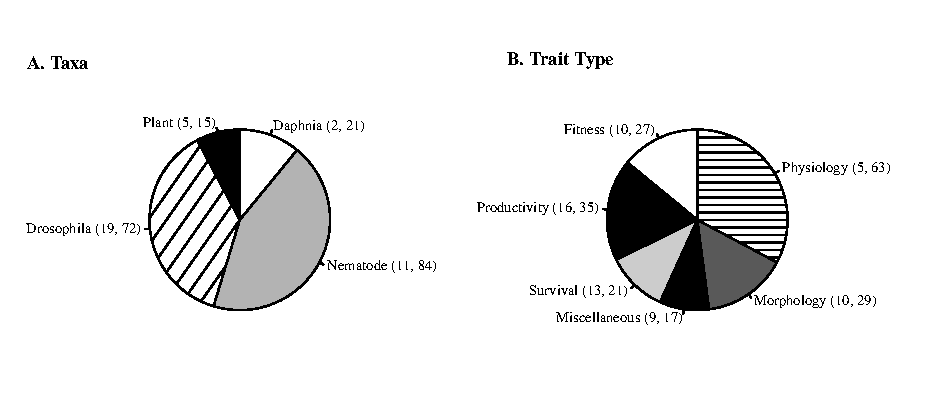
\includegraphics[width=0.9\textwidth]{Chp2_Meta/Fig1Pies_3.02.22.eps}
\caption[The distribution of published mutational variance estimates by taxon (A) and trait (B) categories.]{\textbf{The distribution of published mutational variance estimates by taxon (A) and trait (B) categories.} The number of studies (first value in brackets) and estimates (second value) per category are shown. See Methods (and Table \ref{tab:TraitTypes}) for details of the categories and Table \ref{tab:TabS1} for the studies.} 
\label{fig:Pies}
\end{figure}

\newpage
\FloatBarrier
\begin{figure}
    \centering
    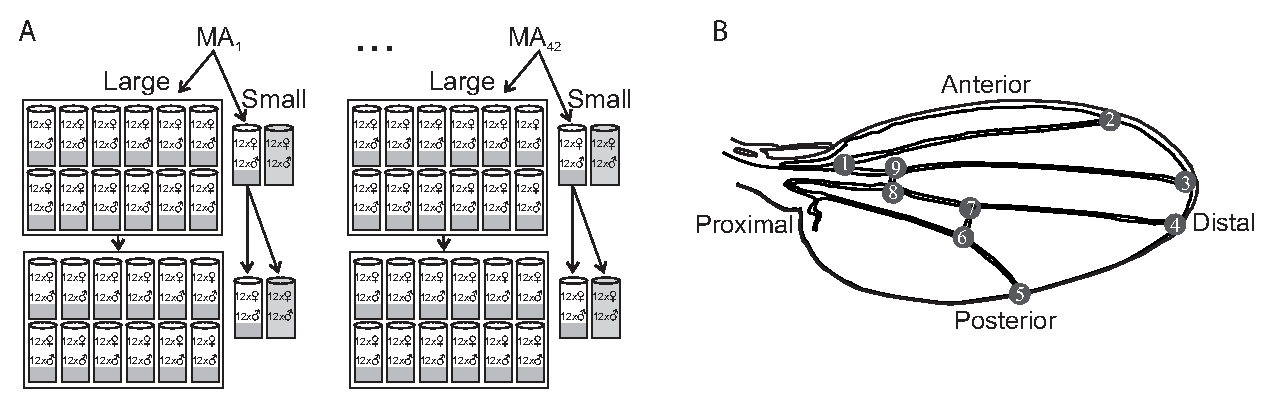
\includegraphics[width=0.9\textwidth]{Chp2_Meta/Fig2.MAdesign.eps}
    \caption[Schematic of design (A) and phenotypes (B) from a manipulative experiment in \textit{Drosophila serrata.} ]{\textbf{Schematic of design (A) and phenotypes (B) from a manipulative experiment in \textit{Drosophila serrata.}}(A) 42 MA lines (evolved through 20 generations of brother-sister mating) each founded two sublines: Small (S; 12 virgin males and 12 virgin females) and Large (L; 144 virgin males and 144 virgin females, distributed evenly among 12 vials). These 84 lines (S and L subline per 42 MA lines) were maintained at these census population sizes for six generations (only two shown here). Each generation, all emergent flies from the 12 vials per L subline were pooled prior to virgin collection. For S sublines, two vials were established each generation; the focal vial contributed offspring to the next generation, while the replicate vial (grey shaded) did not. Each generation, one wing was sampled from each of six randomly chosen males from each of two vials per line (focal and replicate vials for S; randomly chosen two for L). (B) Wing size and shape were characterised from landmarks recorded on an image of each wing: proximal (1) and distal intersections of the radial vein (2); distal intersections of medial (3), cubital vein (4), and distal veins (5) and; the posterior (6, 7) and anterior (8, 9) cross-veins. Inter-landmark distance traits were described by their end-point landmarks (e.g., ILD1.2 was the distance between landmark1 and landmark 2).}
    \label{fig:Fig2MetMRdsgn}
\end{figure}

\newpage
\FloatBarrier
\begin{figure}[!ht]
    \centering
    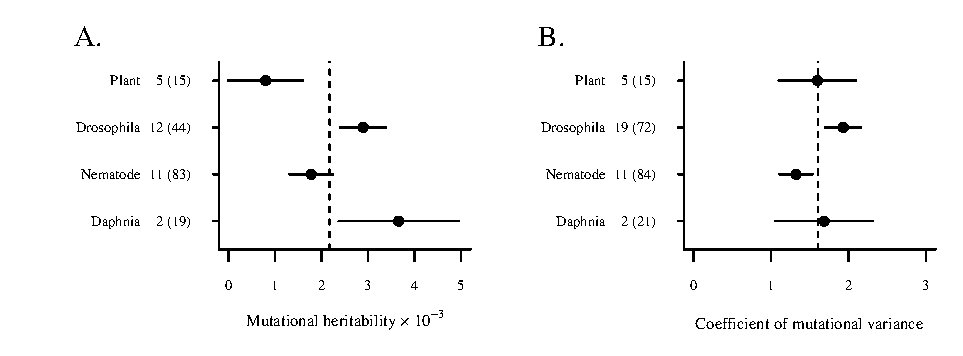
\includegraphics{Chp2_Meta/Fig4_Taxa_LSm.eps}
    \caption[Variation in estimates of (A) mutational heritability and (B) coefficient of mutational variance across taxon categories.]{\textbf{Variation in estimates of (A) mutational heritability and (B) coefficient of mutational variance across taxon categories.} Plotted are the least-squares mean estimates ($\pm$ SE) from the analysis of model (\ref{eqn:metaMM}). The number of studies (and estimates) analysed for each category are shown. The dashed line indicates the global mean value.}
    \label{fig:3TaxaLSM}
\end{figure}

\FloatBarrier
\vspace{5cm}
\begin{figure}[!h]
    \centering
    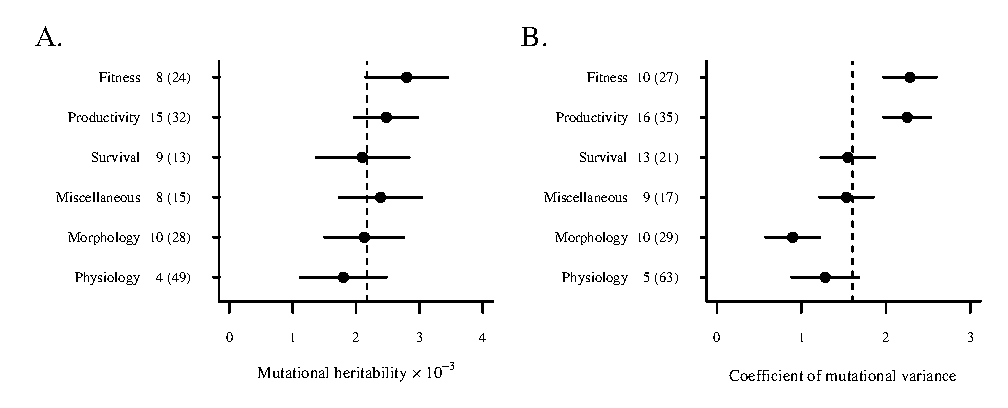
\includegraphics{Chp2_Meta/Fig3_SubTraits_LSm.eps}
    \caption[Variation in estimates of (A) mutational heritability and (B) coefficient of mutational variance across trait categories.]{\textbf{Variation in estimates of (A) mutational heritability and (B) coefficient of mutational variance across trait categories.} Plotted are the least-squares mean estimate ($\pm$ SE) from the analysis of model (\ref{eqn:metaMM}). The number of studies (and estimates) analysed for each category are shown. The dashed line indicates the global mean value.}
    \label{fig:4Subtraits}
\end{figure}

\FloatBarrier
\newpage
\begin{figure}
    \centering
    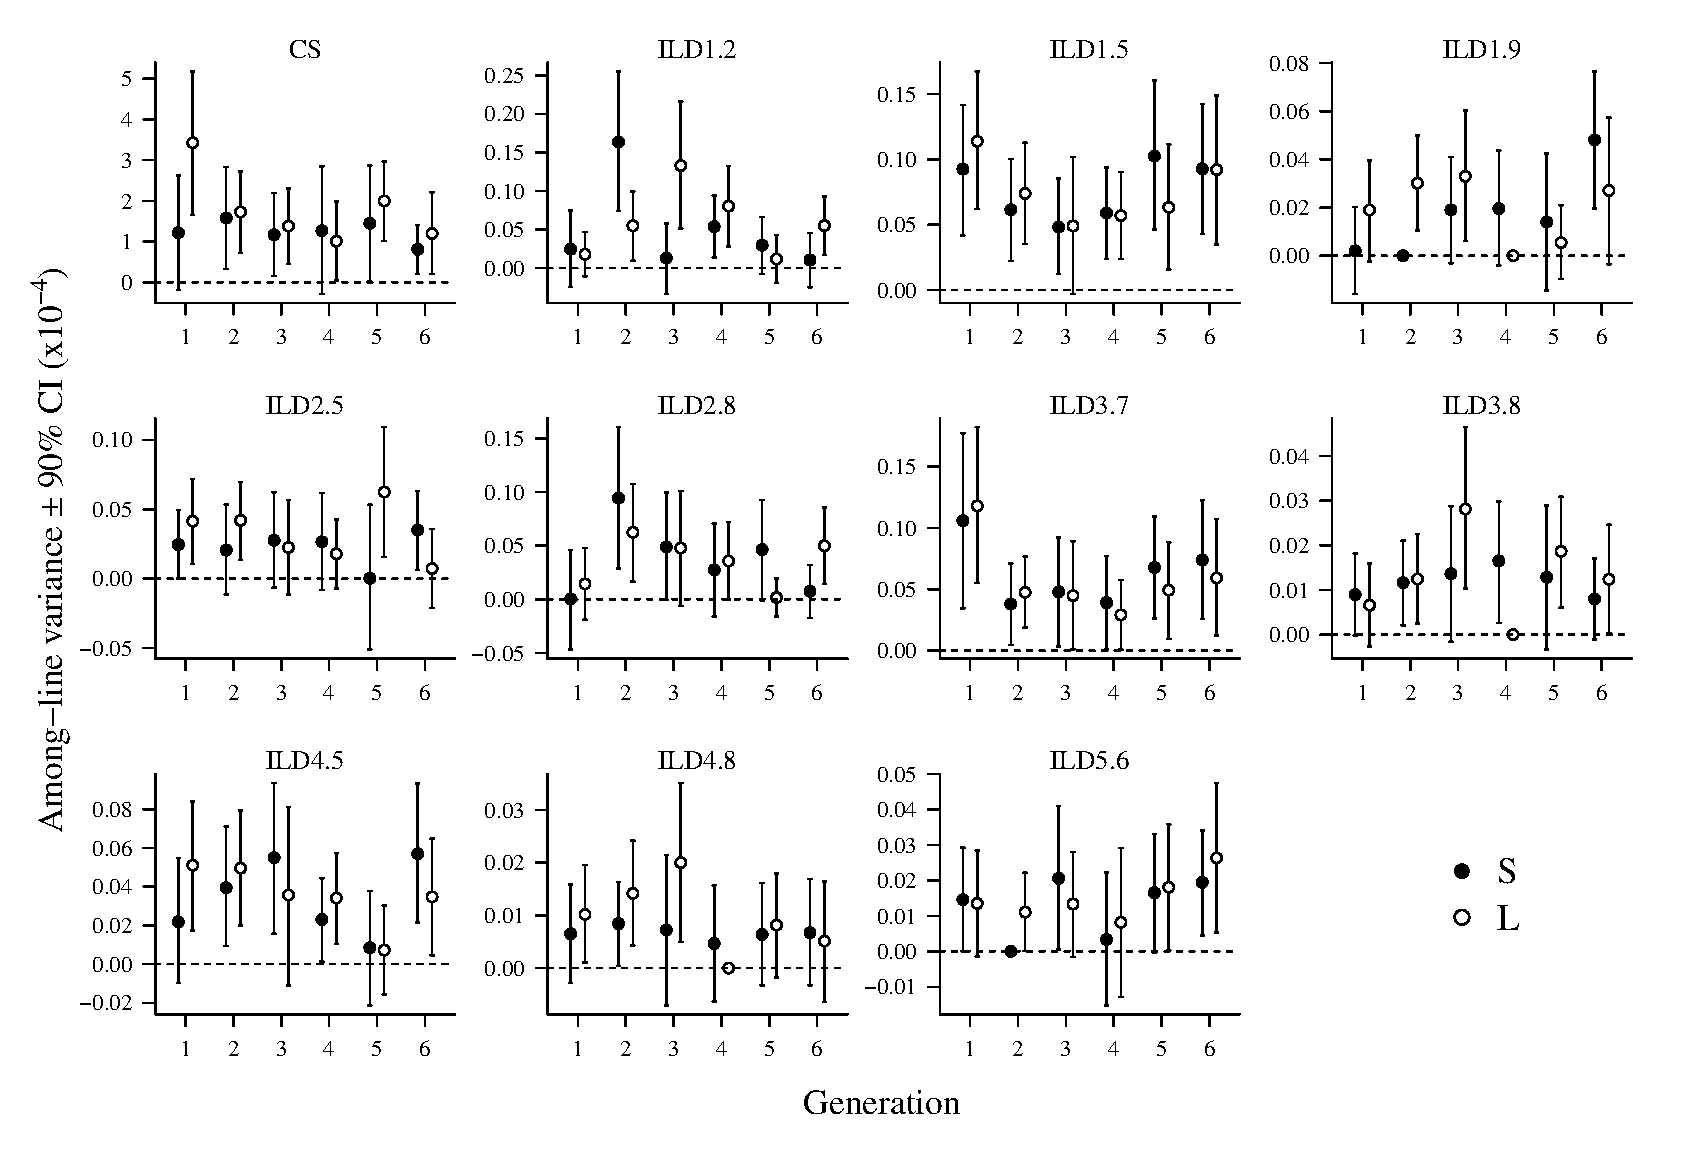
\includegraphics[width=0.9\textwidth]{Chp2_Meta/Fig5VlBounce.eps}
    \caption[Among-line variance estimates across six generations in an experiment in \textit{Drosophila serrata.}]{\textbf{Among-line variance estimates across six generations in an experiment in \textit{Drosophila serrata.}} Variances were estimated independently for each trait (panel; see Figure \ref{fig:Fig2MetMRdsgn}B for trait definitions) in each generation (x-axis) for each of the two population size treatments (Small: solid circles; Large: open circles). Plotted are the REML point estimate, and the REML-MVN 90\% confidence intervals (CI). The dashed horizontal line indicates zero;  estimates for which the lower CI did not overlap zero were interpreted as statistically supported. Where REML estimates of among line variance were zero, no CI are plotted.}
    \label{fig:Fig5VlBounce}
\end{figure}

\FloatBarrier
\newpage
\begin{figure}
    \centering
    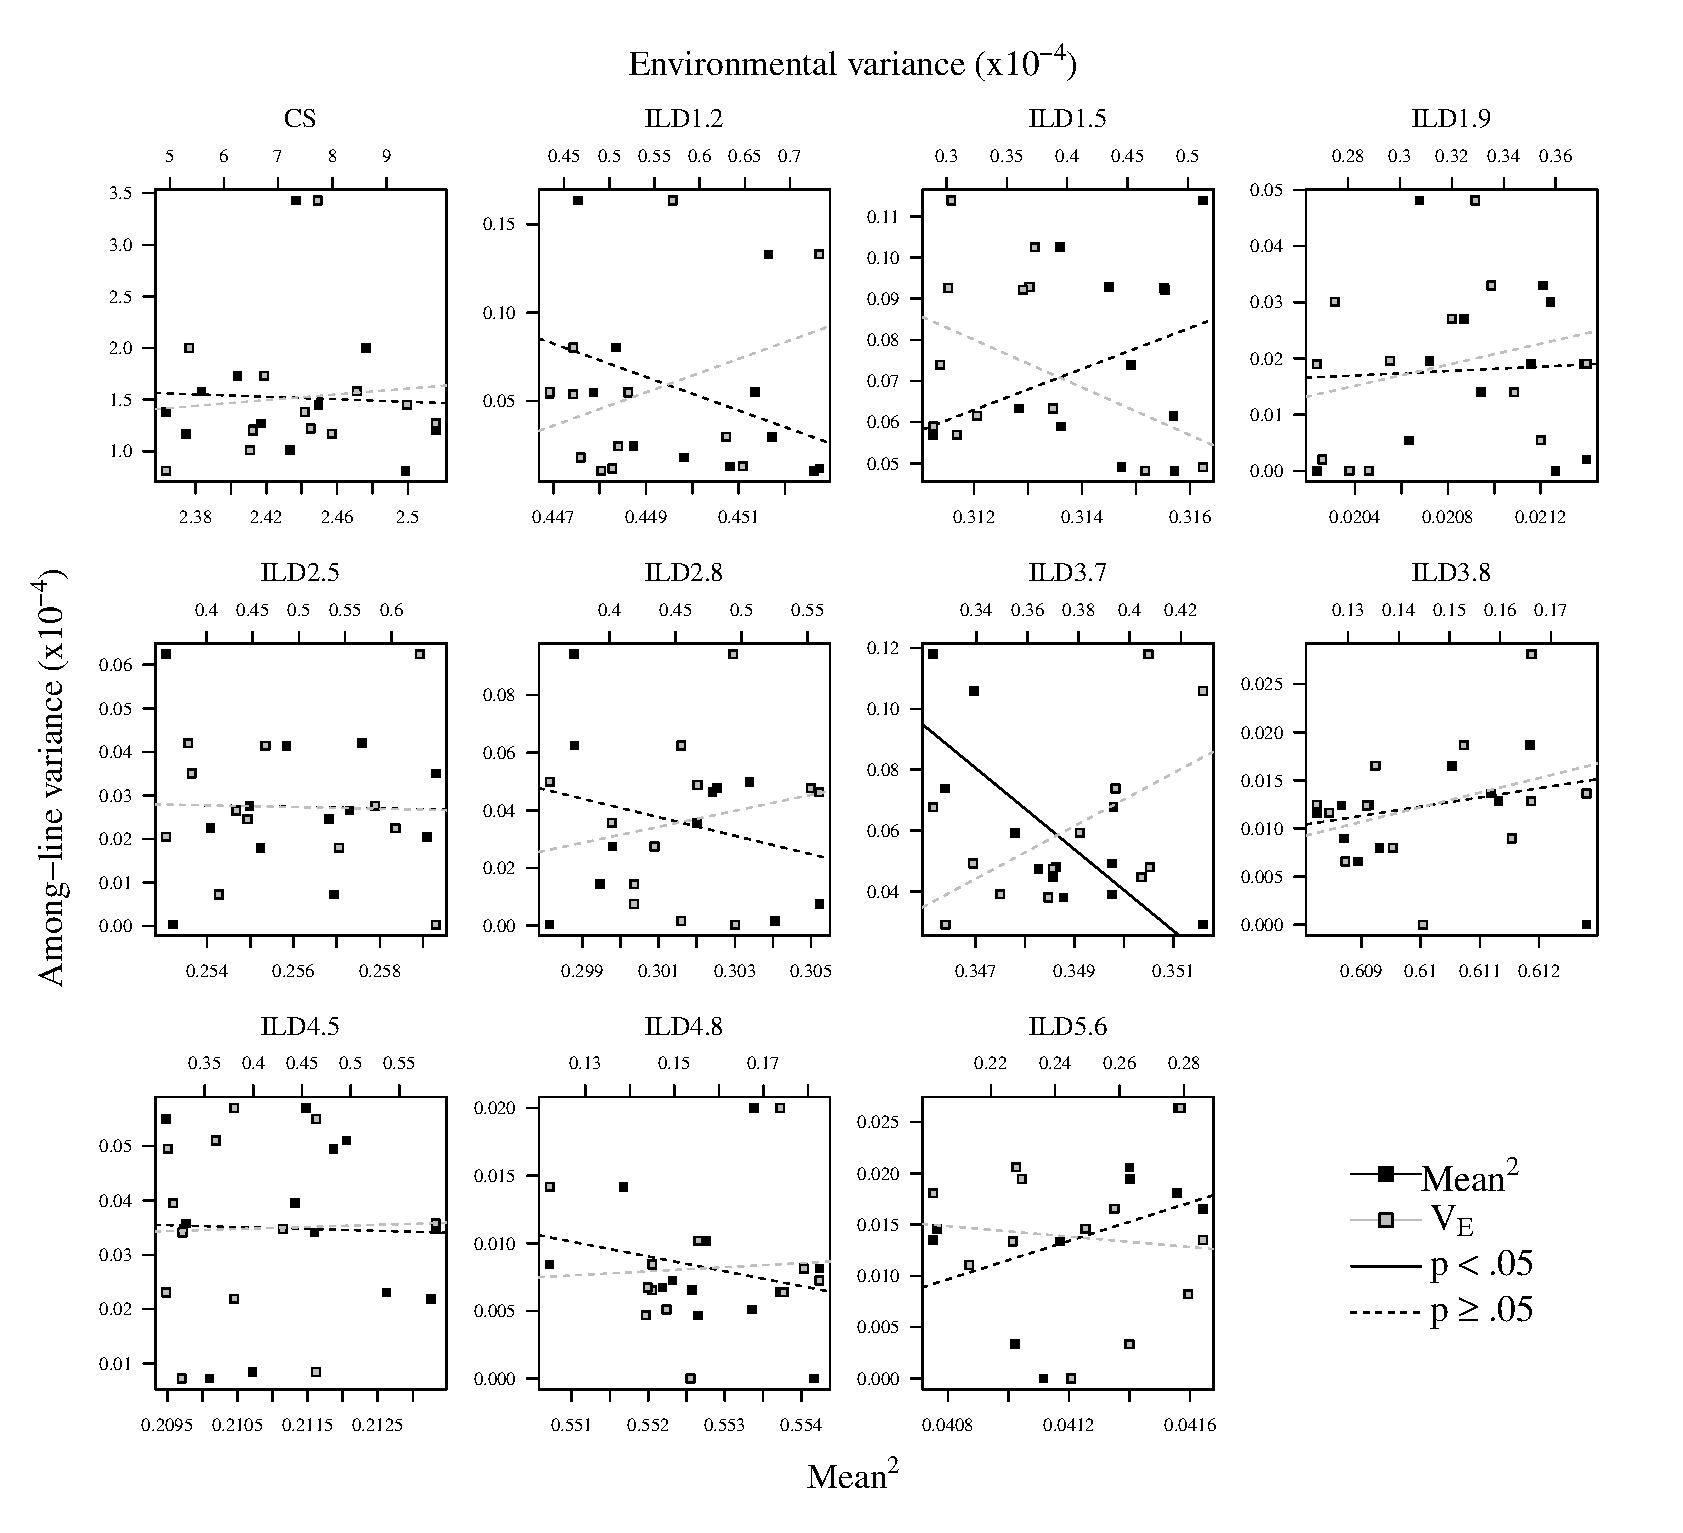
\includegraphics[width=0.9\textwidth]{Chp2_Meta/Fig6VlonPred.eps}
    \caption[Among-line variance estimates for \textit{Drosophila serrata} wing traits plotted as a function of trait mean or variance.]{\textbf{Among-line variance estimates for \textit{Drosophila serrata} wing traits plotted as a function of trait mean or variance.} The 12 estimates of among-line variances for each of the eleven wing traits (panels; see Figure \ref{fig:Fig2MetMRdsgn}B for trait definitions) are plotted against the  corresponding (i.e., same generation and treatment) squared trait mean (bottom x-axis, black symbols) or environmental variance (summed among and within vial variances; top x-axis, grey symbols). All regression statistics are reported in Table S4; only the effect of mean$^2$ on $V_L$ of ILD3.7 was significant at $P < 0.05$, although it does not remain significant after applying a 5\% FDR correction. }
    \label{fig:Fig6Vl_Denom}
\end{figure}



\FloatBarrier
\newpage
\begin{figure}
    \centering
    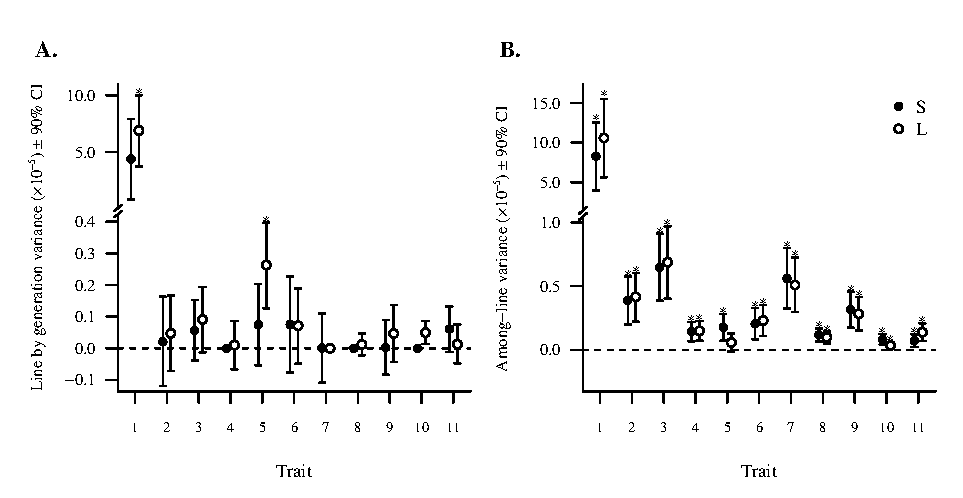
\includegraphics{Chp2_Meta/Fig7_GxE.eps}
    \caption[Estimates of variance from an experiment in \textit{Drosophila serrata.}]{\textbf{Estimates of variance from an experiment in \textit{Drosophila serrata.}} (A) Among-line by generation (G$\times$E) variance and (B) among-line variance estimated for 11 \textit{D. serrata wing} traits (x~-~axis), in two different population size treatments (Small: solid circles; Large: open circles). Plotted are the REML point estimates (from model \ref{eqn:metaVL_GxE}) and the REML-MVN 90\% confidence intervals (CI) around this. The dashed horizontal line indicates zero; statistical significance was inferred where the lower 5\% CI did not overlap zero. After applying a conservative 5\% FDR correction, two estimates in (A) and 21 in (B) remained significant (asterisk above CI).}
    \label{fig:7_GxE}
\end{figure}

\begin{figure}
    \centering
    \includegraphics{Chp2_Meta/elevenVlvsMeanSqdorVE.eps}
    \caption[Among-line variances for eleven wing traits in \textit{Drosophila serrata}.]{\textbf{Among-line variances for eleven wing traits in \textit{Drosophila serrata}.} (A) Among-line variance, $V_L$ REML estimates (and 90\% CI) (model \ref{eqn:metFinMod}; see Figure \ref{fig:Fig2MetMRdsgn}B for trait definitions) are plotted. Dashed line indicates zero. (B) REML estimates of among line variance (points in panel A) were plotted against the corresponding estimate of environmental variance (black circles, top x-axis) or mean squared (grey squares, bottom x-axis) of the trait. Regression results are reported in text.}
    \label{fig:8ElevenVL}
\end{figure}


